\chapter{Uvod}
\label{Chapter1}

Ovaj seminar se bavi statističkim testovima, tj. prihvaćanjem ili odbacivanjem hipoteza. Započinje kratim opisom postupaka testiranja, objašnjavanjem ključnih pojmova te zatim demonstrira postupak testiranja na statističkom testiranju očekivanja.

Početna je premisa jednostavna, imamo hipotezu koju želimo provjeriti. Ona može biti svakojaka:

\begin{itemize}
\item na FERu je 99\% muškaraca 
\item dnevno 1000 studenata FFZG idu u Cassandru
\item Varijanca bodova na SISu je 15
\end{itemize}

Kao što vidimo u primjerima one testiraju vjerojatnost za neki parameter populacije $\Theta$. On može biti različit: postotak pripadnika jedne subpopulacije, broj, očekivanje, varijanca neke statistike i mnoge druge oblike. Za daljnje primjere slučajna varijabla populacije ce biti $X$.

Uzorak nazivamo $n$-torku $(x_1, \ldots, x_n)$ koji su nezavisne realizacije slučajne varijable $X$. One imaju identičnu razdiobu kao i ona.\cite{vis3}

Statistikom nazivamo svaku funkciju koja ovisi o uzorku $X_1 , X_2 , \ldots X_n$ , a ne ovisi (eksplicitno) o nepoznatom parametru kojeg dobivamo iz tog uzorka. \cite{vis3} Vrijednost te statistike naziva se procjenom parametra. \cite{vis3}

Na temelju uzorka iz populacije donosimo zaključke. Budući da sami uzorci podliježu šansi (npr. nas uzorak FERovaca sastoji se od 20 zena no prezentira li to sliku populacije?) želimo znati koliko su sigurne naše pretpostavke. 

Također prilikom uzorkovanja populacije moramo paziti na razne sistematske greške te kako ih izbjegavati. 

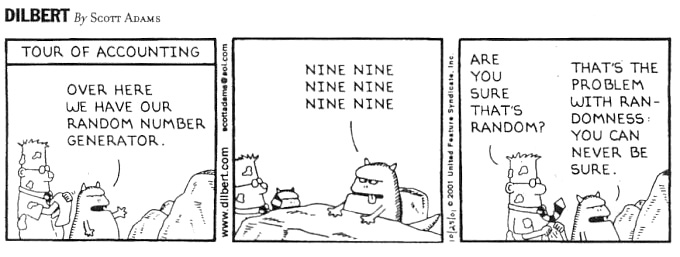
\includegraphics[width=\textwidth]{dilbert.jpg}